Figure \ref{fig:results} shows charge to discharge ratio from the practical system. Compared to the theoretical result shown in figure \ref{fig:crs} (a) a clear degradation can be noticed. The average value has been reduced from 6 to 4.75. This is due to two major reasons, the imperfection of practical components and the assumptions taken in theoretical model. In theoretical model we made the assumption that during the charge cycle there is no current flowing into the battery and $i_r \approx i_c $, where as in reality a small current is flowing into the battery hence producing the non ideality in the actual results.

%---------- Charge to Discharge ratio from the actual circuit
%
\begin{figure}[h!]
\centering
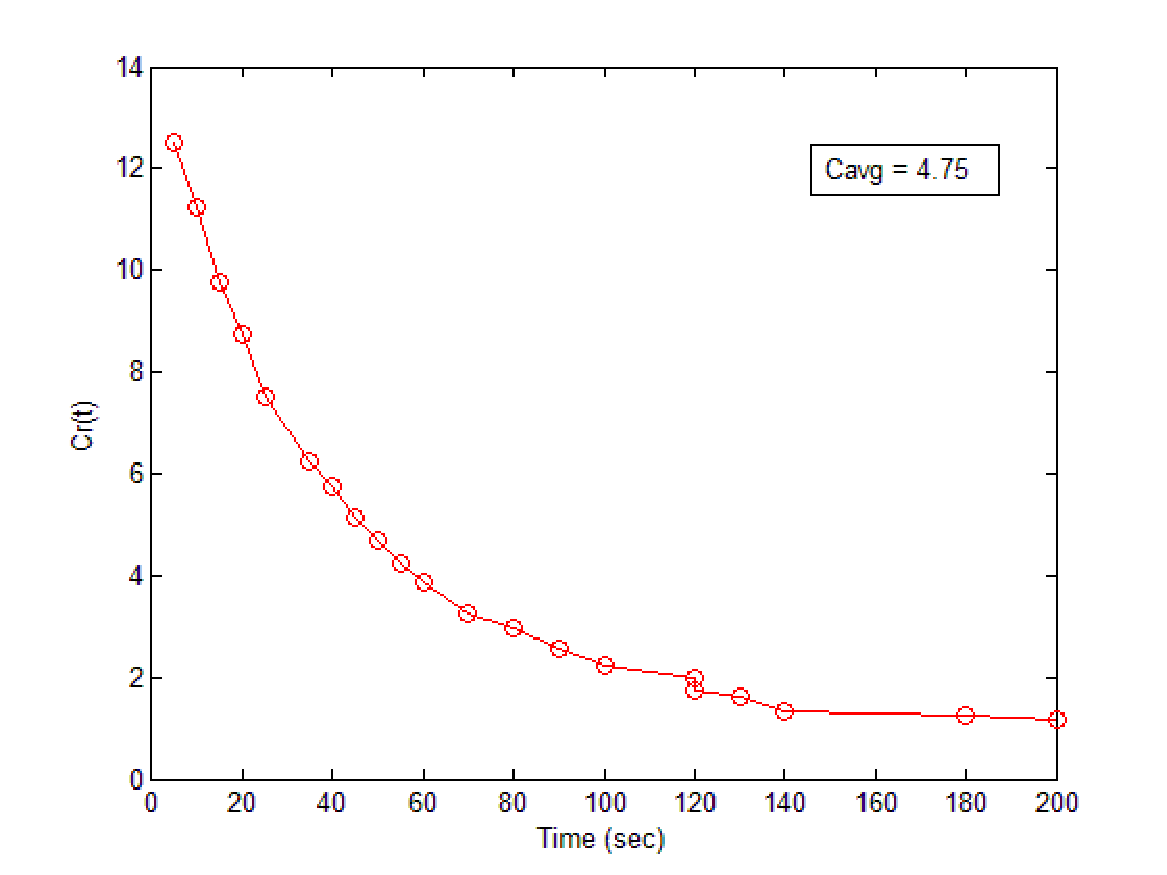
\includegraphics[width=0.8\textwidth]{results.pdf}
\caption{Charge to discharge Ratio}
\label{fig:results}
\end{figure}
%

%---------- The dimension figure goes here

\begin{figure}[h!]
\centering
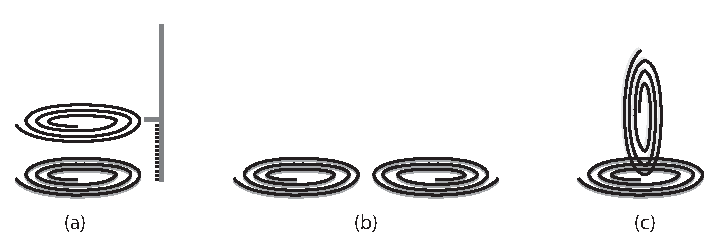
\includegraphics[width=0.9\textwidth]{dimension.pdf}
\caption{Orientations of the test set-up}
\label{fig:dimension}
\end{figure}

%-----------------------Table ----------------------------------------
\begin{tabular*}{\textwidth}{@{\extracolsep{\fill}} |l|l|}
\hline
Distance between two coils (cm) & Efficiency (\%) \\
\hline
0 & 70 \\
1 & 60 \\
2 & 50 \\
3 & 40 \\
4 & 30 \\
\hline
\end{tabular*}
\begin{center}
\textbf{ Table 2.} Distance vs Efficiency
\end{center}
